\documentclass[hyperref, a4paper]{article}

\usepackage{geometry}
\usepackage{titling}
\usepackage{titlesec}
% No longer needed, since we will use enumitem package
% \usepackage{paralist}
\usepackage{enumitem}
\usepackage{footnote}
\usepackage{enumerate}
\usepackage{amsmath, amssymb, amsthm}
\usepackage{mathtools}
\usepackage{bbm}
\usepackage{cite}
\usepackage{graphicx}
\usepackage{subfigure}
\usepackage{physics}
\usepackage{tensor}
\usepackage{siunitx}
\usepackage[version=4]{mhchem}
\usepackage{tikz}
\usepackage{xcolor}
\usepackage{listings}
\usepackage{autobreak}
\usepackage[ruled, vlined, linesnumbered]{algorithm2e}
\usepackage{xr-hyper}
\usepackage[colorlinks,unicode]{hyperref} % , linkcolor=black, anchorcolor=black, citecolor=black, urlcolor=black, filecolor=black
\usepackage{prettyref}

% Page style
\geometry{left=3.18cm,right=3.18cm,top=2.54cm,bottom=2.54cm}
\titlespacing{\paragraph}{0pt}{1pt}{10pt}[20pt]
\setlength{\droptitle}{-5em}
\preauthor{\vspace{-10pt}\begin{center}}
\postauthor{\par\end{center}}

% More compact lists 
\setlist[itemize]{itemindent=17pt, leftmargin=1pt}

% Math operators
\DeclareMathOperator{\timeorder}{\mathcal{T}}
\DeclareMathOperator{\diag}{diag}
\DeclareMathOperator{\legpoly}{P}
\DeclareMathOperator{\primevalue}{P}
\DeclareMathOperator{\sgn}{sgn}
\newcommand*{\ii}{\mathrm{i}}
\newcommand*{\ee}{\mathrm{e}}
\newcommand*{\const}{\mathrm{const}}
\newcommand*{\suchthat}{\quad \text{s.t.} \quad}
\newcommand*{\argmin}{\arg\min}
\newcommand*{\argmax}{\arg\max}
\newcommand*{\normalorder}[1]{: #1 :}
\newcommand*{\pair}[1]{\langle #1 \rangle}
\newcommand*{\fd}[1]{\mathcal{D} #1}
\DeclareMathOperator{\bigO}{\mathcal{O}}

% TikZ setting
\usetikzlibrary{arrows,shapes,positioning}
\usetikzlibrary{arrows.meta}
\usetikzlibrary{decorations.markings}
\tikzstyle arrowstyle=[scale=1]
\tikzstyle directed=[postaction={decorate,decoration={markings,
    mark=at position .5 with {\arrow[arrowstyle]{stealth}}}}]
\tikzstyle ray=[directed, thick]
\tikzstyle dot=[anchor=base,fill,circle,inner sep=1pt]

% Algorithm setting
% Julia-style code
\SetKwIF{If}{ElseIf}{Else}{if}{}{elseif}{else}{end}
\SetKwFor{For}{for}{}{end}
\SetKwFor{While}{while}{}{end}
\SetKwProg{Function}{function}{}{end}
\SetArgSty{textnormal}

\newcommand*{\concept}[1]{{\textbf{#1}}}

% Embedded codes
\lstset{basicstyle=\ttfamily,
  showstringspaces=false,
  commentstyle=\color{gray},
  keywordstyle=\color{blue}
}

\title{Advanced Electrodynamics, Homework 1}
\author{Jinyuan Wu}

\begin{document}

\maketitle

\paragraph{Problem 1} Show that 
\begin{equation}
    \int_{0}^{2 \pi} \int_{0}^{\pi} \vb*{M}_{e m^{\prime} n^{\prime}} \cdot \vb*{M}_{o m n} \sin \theta \mathrm{d} \theta \mathrm{d} \phi=0 ,\quad\text { for all } m, m^{\prime}, n, n^{\prime}.
    \label{eq:prob-1-1}
\end{equation}

\paragraph{Solution} The definition is 
\begin{equation}
    \begin{aligned}
        \vb*{M}_{e m n} &=\frac{-m}{\sin \theta} \sin (m \phi) P_{n}^{m}(\cos \theta) z_{n}(k r) \vu*{e}_{\theta}-\cos (m \phi) \frac{\mathrm{d} P_{n}^{m}(\cos \theta)}{\mathrm{d} \theta} z_{n}(k r) \vu*{e}_{\phi} ,\\
        \vb*{M}_{o m n} &=\frac{m}{\sin \theta} \cos (m \phi) P_{n}^{m}(\cos \theta) z_{n}(k r) \vu*{e}_{\theta}-\sin (m \phi) \frac{\mathrm{d} P_{n}^{m} (\cos \theta)}{\mathrm{d} \theta} z_{n}(k r) \vu*{e}_{\phi}.
        \end{aligned}
\end{equation}
Therefore, we have 
\[
    \begin{aligned}
        &\quad \int_{0}^{2 \pi} \int_{0}^{\pi} \vb*{M}_{e m^{\prime} n^{\prime}} \cdot \vb*{M}_{o m n} \sin \theta \mathrm{d} \theta \mathrm{d} \phi  \\
        &= z_{n'}(kr) z_n(kr) \int_0^{2\pi} \dd{\phi} \int_0^\pi \sin \theta \dd{\theta} \frac{-m' m}{\sin^2 \theta} \sin(m' \phi) \cos(m \phi) P^{m'}_{n'}(\cos\theta) P^m_n(\cos\theta)  \\
        &\quad + z_{n'}(kr) z_n(kr) \int_0^{2\pi} \dd{\phi} \int_0^\pi \sin \theta \dd{\theta} \cos(m' \varphi) \sin(m \varphi) \frac{\mathrm{d} P_{n'}^{m'} (\cos \theta)}{\mathrm{d} \theta} \frac{\mathrm{d} P_{n}^{m} (\cos \theta)}{\mathrm{d} \theta}.
    \end{aligned}
\]
Note that 
\[
    \int_0^{2\pi} \dd{\phi} \sin(m \varphi) \cos(n \varphi) = 0 
\]
for all $m, n \in \mathbb{Z}$, so we have already proved \eqref{eq:prob-1-1}.

\paragraph{}

\paragraph{Problem 2} Suppose that in the basis of vector spherical wave functions, the plane wave 
\begin{equation}
    \boldsymbol{E}=\vu*{\boldsymbol{e}}_{x} E_{0} e^{\mathrm{i} k z}=\vu*{\boldsymbol{e}}_{x} E_{0} e^{\mathrm{i} k r \cos \theta}
    \label{eq:prob-2-4}
\end{equation}
is expanded as 
\begin{equation}
    \vb*{E} = \sum_{m = 0}^\infty \sum_{n = m}^\infty \left( A_{emn} \vb*{N}_{emn}^{(1)} + B_{emn} \vb*{M}_{emn}^{(1)} + A_{omn} \vb*{N}_{omn}^{(1)} + B_{omn} \vb*{M}_{omn}^{(1)} \right).
    \label{eq:prob-2-3}
\end{equation}
The superscript means that in these vector spherical wave functions $z(kr) = j(kr)$.
Prove that 
\begin{equation}
    B_{o 1 n}=\mathrm{i}^{n} E_{0} \frac{2 n+1}{n(n+1)}, \quad A_{e 1 n}=-\mathrm{i} E_{0} \mathrm{i}^{n} \frac{2 n+1}{n(n+1)}.
    \label{eq:prob-2-1}
\end{equation}
Note that 
\begin{equation}
    \hat{\boldsymbol{e}}_{x}=\sin \theta \cos \phi \hat{\boldsymbol{e}}_{r}+\cos \theta \cos \phi \hat{\boldsymbol{e}}_{\theta}-\sin \phi \hat{\boldsymbol{e}}_{\phi},
    \label{eq:prob-2-2}
\end{equation}
each term of which is proportional to $\sin\phi$ or $\cos\phi$, so non-zero vector spherical harmonic components in the expansion are all $m=1$ ones.

\paragraph{Solution} The angular orthogonal relation of vector spherical wave functions gives
\[
    A_{e1n} = \frac{\int_0^{2\pi} \dd{\phi} \int_0^\pi \sin \theta \dd{\theta} \vb*{E} \cdot \vb*{N}^{(1)}_{e1n}}{\int_0^{2\pi} \dd{\phi} \int_0^\pi \sin \theta \dd{\theta} \abs*{\vb*{N}_{e1n}^{(1)}}^2}, \quad B_{o1n} = \frac{\int_0^{2\pi} \dd{\phi} \int_0^\pi \sin \theta \dd{\theta} \vb*{E} \cdot \vb*{M}_{o1n}^{(1)}}{\int_0^{2\pi} \dd{\phi} \int_0^\pi \sin \theta \dd{\theta} \abs*{\vb*{M}^{(1)}_{o1n}}^2}.
\]
We have 
\[
    \begin{aligned}
        B_{o1n} &= \dfrac{\int_0^{2\pi} \dd{\phi} \int_0^\pi \sin \theta \dd{\theta} \vb*{E} \cdot \vb*{M}_{o1n}^{(1)}}{\int_0^{2\pi} \dd{\phi} \int_0^\pi \sin \theta \dd{\theta} \abs*{\vb*{M}^{(1)}_{o1n}}^2} \\
        &= E_0 \frac{\displaystyle \int_0^{2\pi} \dd{\phi} \int_0^\pi \sin \theta \dd{\theta} \ee^{\ii k r \cos \theta} \left( \frac{\cos\phi}{\sin\theta} P^1_n(\cos\theta) \cos\theta \cos\phi - \sin\phi \dv{P^1_n(\cos\theta)}{\theta} (-\sin\phi) \right)}{\displaystyle j_n(kr) \int_0^{2\pi} \dd{\phi} \int_0^\pi \sin \theta \dd{\theta} \left( \frac{1}{\sin^2 \theta} \cos^2\phi (P^1_n(\cos \theta))^2 + \sin^2\phi \left( \dv{P_n^1(\cos\theta)}{\theta} \right)^2 \right) }.
    \end{aligned}
\]
Integrating $\phi$ and we have 
\begin{equation}
    B_{o1n} = E_0 \frac{\displaystyle \int_0^\pi \dd{\theta} \ee^{\ii k r \cos \theta} \left( P^1_n(\cos\theta) \cos\theta + \dv{P^1_n(\cos\theta)}{\theta} \sin \theta \right)}{\displaystyle j_n(kr) \int_0^\pi \sin \theta \dd{\theta} \left( \frac{1}{\sin^2 \theta} (P^1_n(\cos \theta))^2 + \left( \dv{P_n^1(\cos\theta)}{\theta} \right)^2 \right) }.
    \label{eq:b-o1n-1}
\end{equation}
By the same way we can prove that 
\begin{equation}
    B_{e1n} = 0
    \label{eq:be1n-0}
\end{equation}
since the corresponding integrals contain $\int_0^{2\pi} \dd{\phi} \sin\phi \cos\phi$ factors and therefore vanish.
The numerator of \eqref{eq:b-o1n-1} is
\[
    \begin{aligned}
        &\quad \int_0^\pi \dd{\theta} \ee^{\ii k r \cos \theta} \left( P^1_n(\cos\theta) \cos\theta + \dv{P^1_n(\cos\theta)}{\theta} \sin \theta \right) \\
        &= \int_0^\pi \dd{\theta} \ee^{\ii k r \cos \theta} \left( \sqrt{1 - \cos^2\theta} \dv{P_n(\cos\theta)}{\cos \theta } \cos\theta + \sin \theta \dv{\theta} \left( \sqrt{1 - \cos^2\theta} \dv{P_n(\cos\theta)}{\cos \theta }  \right) \right) \\
        &= \int_0^\pi \dd{\theta} \ee^{\ii k r \cos \theta} \left( \sin\theta \dv{P_n(\cos\theta)}{\cos \theta } \cos\theta + \sin \theta \left( \cos\theta \dv{P_n(\cos\theta)}{\cos\theta} - \sin^2\theta \dv[2]{P_n(\cos\theta)}{\cos\theta} \right) \right) \\
        &= \int_{-1}^1 \dd{x} \ee^{\ii k r x} \left( 2 x \dv{P_n(x)}{x} + (x^2 - 1) \dv[2]{P_n(x)}{x} \right) \\
        &= n(n+1) \int_{-1}^1 \dd{x} \ee^{\ii k r x} P_n(x).
    \end{aligned}
\] 
The last line is obtained by the definition of Legendre's polynomials.
By the formula 
\begin{equation}
    j_{n}(\rho)=\frac{\mathrm{i}^{-n}}{2} \int_{0}^{\pi} e^{\mathrm{i} \rho \cos \theta} P_{n}(\cos \theta) \sin \theta \mathrm{d} \theta = \frac{\ii^{-n}}{2} \int_{-1}^1 \dd{x} \ee^{\ii \rho x} P_n(x) ,
    \label{eq:integral-formula-1}
\end{equation}
the numerator of \eqref{eq:b-o1n-1} can be further evaluate as 
\[
    \frac{2}{\ii^{-n}} n(n+1) j_n(kr),
\]
so \eqref{eq:b-o1n-1} reads
\begin{equation}
    \begin{aligned}
        B_{o1n} &= E_0 \frac{n(n+1) j_n(kr)}{\displaystyle \frac{\ii^{-n}}{2} j_n(kr) \int_0^\pi \sin \theta \dd{\theta} \left( \frac{1}{\sin^2 \theta} (P^1_n(\cos \theta))^2 + \left( \dv{P_n^1(\cos\theta)}{\theta} \right)^2 \right) } \\
        &= E_0 \frac{n(n+1)}{\displaystyle \frac{\ii^{-n}}{2}  \int_0^\pi \sin \theta \dd{\theta} \left( \frac{1}{\sin^2 \theta} (P^1_n(\cos \theta))^2 + \left( \dv{P_n^1(\cos\theta)}{\theta} \right)^2 \right) }.
    \end{aligned}
\end{equation}
By integral formulae 
\[
    \int_{-1}^1 \dd{x} \left( \dv{P_n(x)}{x} \right)^2 = \int_{-1}^1 \dd{x} \left( \frac{1}{\sqrt{1 - x^2}} P_n^1(x) \right)^2 = n(n+1)
\]
and 
\[
    \int_{-1}^1 \dd{x} \left( \dv{P^1_n(x)}{x} \right)^2 (1 - x^2) = \frac{n(n+1)(2n^2-1)}{2n+1},
\]
we have 
\[
    \begin{aligned}
        B_{o1n} &= \frac{2 \ii^n E_0 n(n+1)}{n(n+1) + n(n+1) \frac{2n^2 - 1}{2n+1}} \\
        &= \frac{\ii^n (2n+1) E_0 }{n(n+1)},
    \end{aligned}
\]
and hence we have shown the first equation in \eqref{eq:prob-2-1}.

We than evaluate $A_{e1n}$ and $A_{o1n}$. The definition of $\vb*{N}$ functions are
\begin{equation}
    \begin{aligned}
        \boldsymbol{N}^{(1)}_{e 1 n}=& \frac{j_{n}(k r)}{k r} \cos \phi n(n+1) P_{n}^{1}(\cos \theta) \vu*{e}_{r} +\cos \phi \frac{\mathrm{d} P_{n}^{1}(\cos \theta)}{\mathrm{d} \theta} \frac{1}{k r} \frac{\mathrm{d}}{\mathrm{d}(k r)}\left[(k r) j_{n}(k r)\right] \vu*{e}_{\theta}  \\
        &\quad - \sin  \phi \frac{P_{n}^{1}(\cos \theta)}{\sin \theta} \frac{1}{k r} \frac{\mathrm{d}}{\mathrm{d}(k r)}\left[(k r) z_{n}(k r)\right] \hat{e}_{\phi}, \\
        \boldsymbol{N}^{(1)}_{o 1 n}=& \frac{j_{n}(k r)}{k r} \sin \phi n(n+1) P_{n}^{1}(\cos \theta) \vu*{e}_{r} +\sin \phi \frac{\mathrm{d} P_{n}^{1}(\cos \theta)}{\mathrm{d} \theta} \frac{1}{k r} \frac{\mathrm{d}}{\mathrm{d}(k r)}\left[(k r) j_{n}(k r)\right] \vu*{e}_{\theta} \\
        &\quad + \sin \phi \frac{P_{n}^{1}(\cos \theta)}{\sin \theta} \frac{1}{k r} \frac{\mathrm{d}}{\mathrm{d}(k r)}\left[(k r) z_{n}(k r)\right] \hat{e}_{\phi} .
        \end{aligned}
\end{equation}
By \eqref{eq:prob-2-2} we find that 
\begin{equation}
    A_{o1n} = 0,
    \label{eq:ao1n-0}
\end{equation}
as $\sin \phi$ and $\cos \phi$ are orthogonal. Now we consider the $\vu*{e}_r$ component, i.e.
\[
    \sin\theta \cos\phi E_0 \ee^{\ii k r \cos\theta} = \sum_n A_{e1n} n(n+1) \frac{j_n(kr)}{kr} \cos \phi P_{n}^{1}(\cos \theta),
\] 
as $\vb*{M}$ functions do not have $\vu*{e}_r$ components.
Therefore, we have 
\begin{equation}
    \begin{aligned}
        \int_{-\pi}^\pi \dd{\theta} \sin^2\theta E_0 \ee^{\ii k r \cos\theta} P_m^1(\cos\theta) &= \sum_n \int_{-\pi}^\pi \sin\theta \dd{\theta} n(n+1) A_{e1n} \frac{j_n(kr)}{kr} P_n^1(\cos\theta) P_m^1(\cos\theta) \\
        &= \sum_n n(n+1) A_{e1n} \frac{j_n(kr)}{kr} \int_{-1}^1 \dd{x} P_n^1(x) P_m^1(x) \\
        &= m(m+1) A_{e1m} \frac{j_m(kr)}{kr} \frac{2m (m+1)}{2m+1},
    \end{aligned}
    \label{eq:ae1m-step-1}
\end{equation}
where we have used the formula that 
\[
    \int^1_{-1} P^1_m(x) P^1_n(x) \dd{x} = \frac{2 n (n+1)}{2n+1} \delta_{mn}.
\]
Now we just need to evaluate the LHS and then we can find $A_{e1n}$.
We have 
\begin{equation}
    \begin{aligned}
        \int_{-\pi}^\pi \dd{\theta} \sin^2\theta E_0 \ee^{\ii k r \cos\theta} P_m^1(\cos\theta) &= E_0 \int_{-1}^1 \dd{x} \sqrt{1-x^2} \ee^{\ii k r x} P_m^1(x) \\
        &= E_0 \int_{-1}^1 \dd{x} \sqrt{1-x^2} \ee^{\ii k r x} \sqrt{1-x^2} \dv{P_m(x)}{x} \\
        &= E_0 \int_{-1}^1 \dd{x} (1-x^2) \ee^{\ii k r x} \dv{P_m(x)}{x} \\
        &= E_0 \int_{-1}^1 \dd{x} \ee^{\ii k r x} m(x P_m(x) - P_{m-1}(x)) \\
        &= E_0 \int_{-1}^1 \dd{x} \ee^{\ii k r x} \frac{m(m+1)}{2m+1} (P_{m+1}(x) - P_{m-1}(x)),
    \end{aligned}
    \label{eq:ae1m-step-2}
\end{equation}
where we have used the formulae that 
\[
    \frac{x^2 - 1}{n} \dv{P_n(x)}{x} = x P_n - P_{n-1}
\]
and 
\[
    x P_n(x) = \frac{1}{2n+1} \left( n P_{n-1}(x) + (n+1) P_{n+1}(x) \right).
\]
Using \eqref{eq:integral-formula-1} in \eqref{eq:ae1m-step-2}, we have 
\begin{equation}
    \begin{aligned}
        &\quad E_0 \int_{-1}^1 \dd{x} \ee^{\ii k r x} \frac{n(n+1)}{2n+1} (P_{n+1}(x) - P_{n-1}(x)) \\
        &= E_0 \frac{n(n+1)}{2n+1} \left( \frac{2}{\ii^{-n-1}} j_{n+1}(kr) - \frac{2}{\ii^{-n+1}} j_{n-1}(kr) \right) \\
        &= E_0 \frac{n(n+1)}{2n+1} \left( \frac{2}{\ii^{-n-1}} j_{n+1}(kr) + \frac{2}{\ii^{-n-1}} j_{n-1}(kr) \right) \\
        &= E_0 \frac{n(n+1)}{2n+1} \frac{2}{\ii^{-n-1}} \frac{2n+1}{kr} j_n(kr),
    \end{aligned}
    \label{eq:ae1m-step-3}
\end{equation}
where we have used the fact that 
\[
    j_{n-1}(x) + j_{n+1}(x) = \frac{2n+1}{x} j_n(x),
\]
which is a consequence of 
\[
    J_{n-1}(x) + J_{n+1}(x) = \frac{2n}{x} J_n(x)
\]
and 
\[
    j_n(x) = \sqrt{\frac{\pi}{2x}} J_{n+1/2}(x).
\]
Putting \eqref{eq:ae1m-step-1}, \eqref{eq:ae1m-step-2} and \eqref{eq:ae1m-step-3} together, we have 
\[
    m(m+1) A_{e1m} \frac{j_m(kr)}{kr} \frac{2m (m+1)}{2m+1} = E_0 \frac{m(m+1)}{2m+1} \frac{2}{\ii^{-m-1}} \frac{2m+1}{kr} j_n(kr),
\]
or 
\[
    A_{e1m} = - \ii \frac{(2m+1) \ii^m E_0}{m(m+1)},
\]
which is the second equation in \eqref{eq:prob-2-1}.

So now we have completed a proof of \eqref{eq:prob-2-1}, and since we also have \eqref{eq:prob-2-3}, \eqref{eq:be1n-0} and \eqref{eq:ao1n-0}, we now have expanded the plane wave \eqref{eq:prob-2-4} into 
\begin{equation}
    \boldsymbol{E}=E_{0} \sum_{n=1}^{\infty} \mathrm{i}^{n} \frac{2 n+1}{n(n+1)} \left( \boldsymbol{M}_{o 1 n}^{(1)}-\mathrm{i} \boldsymbol{N}_{e 1 n}^{(1)} \right).
    \label{eq:prob-2-5}
\end{equation}

\paragraph{}

\begin{figure}
    \centering
    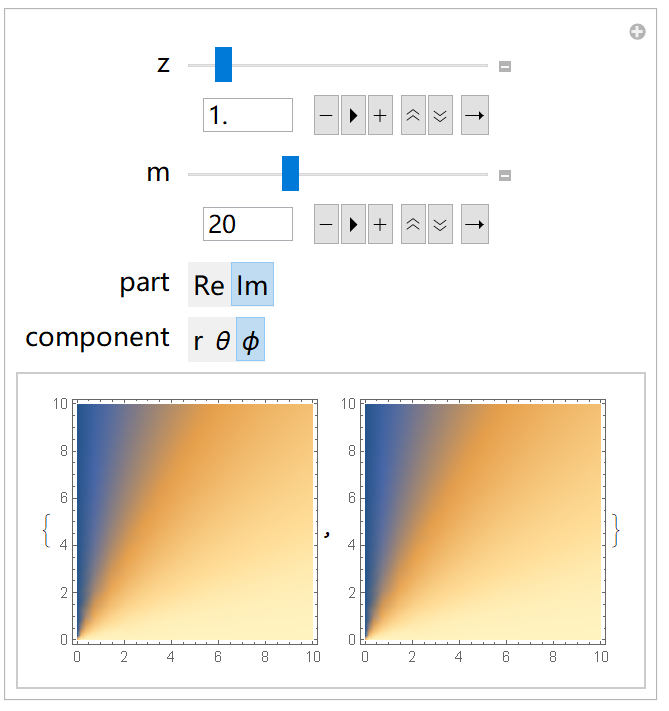
\includegraphics[width = 0.6\textwidth]{example-ui.PNG}
    \caption{Numerical demonstration of \eqref{eq:prob-2-5}. The left figure is the RHS and the right figure is the LHS. $m$ should be greater than 10 to achieve a good approximation.}
    \label{fig:example-ui}
\end{figure}

\paragraph{Problem 3} Verify numerically the expansion \eqref{eq:prob-2-5}. 

\paragraph{Solution} Since visualizing a 3D vector field is hard, we will work on its three components in spherical coordinates and the real and imaginary parts one by one.

The result can be found \href{./homework-1-numerical.nb}{toghether with this document}, where we plot the RHS of \eqref{eq:prob-2-5} with a fixed $z$.
The parameters - the maximum of $n$ in the summation in \eqref{eq:prob-2-5} (labeled as $m$), $z$, which components to be shown and whether to show the real part or the imaginary part - can be changed interactively.
An example can be found in \eqref{fig:example-ui}.

\end{document}